\documentclass{article}
\usepackage{graphicx} % Required for inserting images
\usepackage[a4paper, margin=1in]{geometry}
\usepackage{amsmath}
\parindent 0pt

\title{Motors, Buoyancy and Boat Load}
\author{Hritik Roy Chowdhury}
\date{October 2023}

\parindent 0pt

\begin{document}

\maketitle

\vspace{2cm}
\begin{center}
    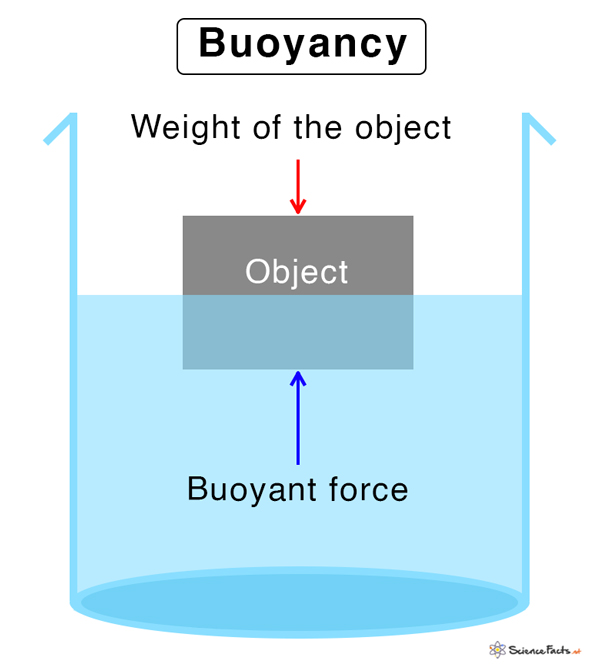
\includegraphics[width=0.75\textwidth]{Buoyancy.jpg}
\end{center}

\newpage

\section*{Preface}
After researching formulas and theory behind propellers in liquids, thrust and more, it seems almost impossible to do any calculations for thrust and power requirements. Here's why:
\begin{itemize}
    \item We don't know what the efficiency of the motor or the propellers are
    \item We don't know how much thrust the motors will produce. To find the thrust, you also need variables such as the water speed coming into the motors.
    \item We don't know the dimensions/size/shape of the propellers which heavily affect the thrust
\end{itemize}
Overall, it is very cumbersome to calculate the power needed for the boat to move with a certain maximum load. It is therefore enough to simply order appropriately powerful and waterproof motors and observe the performance from there. \\

The boat will obviously move from whatever motor we find. The more powerful the motor is, the faster the boat will move. So, it is not necessary to determine motor power outputs as any motor would create a force to move the boat. \\

Now, to find the maximum weight that the boat can take (load), we would also need to find the buoyancy force of the water on the boat. However, this is not possible until the actual boat is made to test the displacement volume on water (see \ref{introduction}). On the other hand, a rough estimation can be made which should be quite an accurate model of determining the maximum load of the boat. Determining a value for the maximum load is explored in this report.

\newpage

\section*{Introduction}
\label{introduction}

The buoyancy force from the water on the boat is given by,
$$F_B=\rho gV$$
where $V$ is the \textbf{volume of the boat that is submerged under water} while it floats. The density of water is $\rho$ and $g$ is the gravitational acceleration. \\

Let's assume that for the maximum buoyancy force, we take the whole boat's volume to be $V$ (i.e the submerged volume is taken as if the boat is underwater). If $l, w$ and $h$ are the length, width and height of the boat, respectively, simplified to a cuboid, and realistic values are chosen for these, then,
$$V=l\cdot w\cdot h=0.5\ \mathrm{m}\cdot 0.35\ \mathrm{m}\cdot 0.2\ \mathrm{m}=0.035\ \mathrm{m^3}$$
Notice that this is a decently big boat. The buoyancy force is,
$$F_B=1000\ \mathrm{kg\ m^{-3}}\cdot9.82\ \mathrm{m\ s^{-2}}\cdot0.035\ \mathrm{m^3}=343.7\ \mathrm{N}$$
Hence, any load larger than this will cause the boat to sink. \\[1cm]

\section*{Realistic Approximation}

Realistically, our boat will probably have a submerged volume of approximately,
$$V=l\cdot w\cdot h=0.5\ \mathrm{m}\cdot 0.35\ \mathrm{m}\cdot 0.07\ \mathrm{m}=0.01225\ \mathrm{m^3}$$
Here, the height of the boat submerged underwater is now only $7\ \mathrm{cm}$ which is more realistic. In such a case, the realistic buoyancy force is,
$$F_B=1000\ \mathrm{kg\ m^{-3}}\cdot9.82\ \mathrm{m\ s^{-2}}\cdot0.01225\ \mathrm{m^3}\doteq120\ \mathrm{N}$$
Assuming that the boat weighs a maximum of $2\ \mathrm{kg}$, the remaining load can be calculated. The buoyancy force, $F_B$ must always be larger than the total weight of the boat (including load and boat weight) or else it will sink. So,
\begin{align*}
    F_B&>Mg \\ 
    F_B&>(m_{\mathrm{boat}}+m_{\mathrm{load}})g \\
    120\ \mathrm{N}&>(2\ \mathrm{kg}+m_{\mathrm{load}})g \\
    \frac{120\ \mathrm{N}}{g}-2\ \mathrm{kg}&>m_{\mathrm{load}}
\end{align*}
Hence, the maximum load that the boat can take is,
$$m_{\mathrm{load}}=\frac{120\ \mathrm{N}}{9.82\ \mathrm{m s^{-2}}}-2\ \mathrm{kg}=\textbf{10.2 kg}$$
Do note, that the submerged height here is taken to be $7\ \mathrm{cm}$. However, it is almost certain that our model will have a higher value for this which will result in a higher buoyancy force, and so, a higher maximum load.

\end{document}
